\documentclass{standalone}
%outline around text
\usepackage[outline]{contour}
\contourlength{1.3pt}

%tikz
\usepackage{tikz}
\usetikzlibrary{knots, cd, calc}

\begin{document}


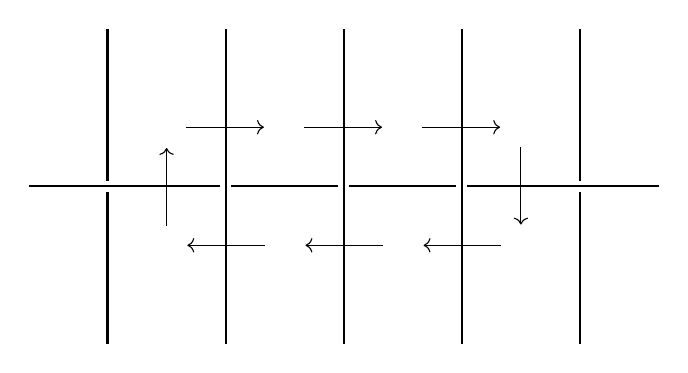
\begin{tikzpicture}[yscale=1]
\begin{knot}[clip width = 5]

\strand[thick] (2.5, -2) -- (2.5, 2);
\strand[thick] (4, -2) -- (4, 2);
\strand[thick] (5.5, -2) -- (5.5, 2);

\strand[thick] (0, 0) -- (8, 0);

\strand[thick] (1, -2) -- (1, 2);
\strand[thick] (7, -2) -- (7, 2);

\strand[->] (2, 0.75) -- (3, 0.75);
\strand[->] (3.5, 0.75) -- (4.5, 0.75);
\strand[->] (5, 0.75) -- (6, 0.75);
\strand[->] (6, -0.75) -- (5, -0.75);
\strand[->] (4.5, -0.75) -- (3.5, -0.75);
\strand[->] (3, -0.75) -- (2, -0.75);
\strand[->] (1.75, -0.5) -- (1.75, 0.5);
\strand[->] (6.25, 0.5) -- (6.25, -0.5);
\end{knot}
\end{tikzpicture}



\end{document}